%
% Modified by Sameer Vijay
% Last Change: Wed Jul 27 2005 13:00 CEST
%
%%%%%%%%%%%%%%%%%%%%%%%%%%%%%%%%%%%%%%%%%%%%%%%%%%%%%%%%%%%%%%%%%%%%%%%%
%
% Sample Notre Dame Thesis/Dissertation
% Using Donald Peterson's ndthesis classfile
%
% Written by Jeff Squyres and Don Peterson
%
% Provided by the Information Technology Committee of
%   the Graduate Student Union
%   http://www.gsu.nd.edu/
%
% Nothing in this document is serious except the format.  :-)
%
% If you have any suggestions, comments, questions, please send e-mail
% to: ndthesis@gsu.nd.edu
%
%%%%%%%%%%%%%%%%%%%%%%%%%%%%%%%%%%%%%%%%%%%%%%%%%%%%%%%%%%%%%%%%%%%%%%%%

%
% Chapter 4
%

\chapter{DATA ANALYSIS}
\label{chap:dataAnalysis}
\begin{comment}
We care about two things:
1. The absolute cross-section of the ground state transition
2. Setting a limit on excited 0+ state cross-sections
\end{comment}
The aim of the data analysis of the \reaction data sets is to extract the absolute cross-section of the reaction populating the ground state of \GeTargets and also to set a limit on excited \zp state cross-sections.  Each of these analyses is discussed in its own section, but because the absolute cross-section is of interest, the detector efficiency and several properties of the experiment must be accurately determined.  The detector efficiency is discussed first.

\section{Detector Efficiency}
\begin{comment}
deuterium, Mg, cuts
\end{comment}
The measurement made by the neutron detector is counts - counts of neutrons of differing energies.  The number of counts due to neutrons made by the neutron detector scales linearly with the absolute cross-section of \reaction but is not identical to it because not all the neutrons produced leave a signal in the detector.  The ratio of the detected neutron flux to the total neutron flux is called the efficiency of a detector and must be carefully determined as its error contributes directly to the systematic uncertainty of the extracted absolute cross-sections.

The efficiency of a plastic-scintillator-type neutron detector depends on its size and shape as well as the energy resolution and the detection threshold.  The Monte-Carlo code of Cecil \cite{Cecil_neutEfficiency} can calculate the efficiency of a plastic scintillator detector.  These calculations match measured efficiency values well over a wide range of neutron energies.  The inputs required by the code are the density of the detector, its H/C ratio, the threshold used in the experiment, and the interval over which the detector averages the neutron energy, i.e., the resolution of the detector.  The plastic properties have been reported in {\tab}??, and the threshold and resolution of the detector must be determined with data from the experiment.  

Efficiency calculations were performed with several data sets to ensure that the Cecil code accurately predicted the efficiency of the neutron detector.  Ideal test reactions are those with well-known cross-sections and neutrons with energies near 26~MeV.  The reaction d(d,n) has been well-measured at beam energies of 9~MeV, giving neutrons with ??~MeV.  The estimated efficiency gives a cross-section that matches well with the published value, as shown in {\fig}~\ref{fig:DeuteriumMatch}.  The \MgReaction has not been measured at a beam energy of 16~MeV but has been measured at lower and higher energies as shown in  {\tab}~\ref{tab:efficiencyCalib}.  The efficiency measured for the neutrons from this reaction provides a measurement very near the energies produced in \reaction and can be checked against previous measurements.  {\fig} shows the light output used to determine the resolution and threshold needed by the code, and {\fig} shows the consistency of the measured cross-section using that predicted efficiency.  Because the efficiency of the detector changes very slowly at these neutron energies, this efficiency was used for all bars for the \MgReaction and \reaction data sets.


\section{Experimental Parameters Related to the Cross Section}
\begin{comment}
current, tgt thickness (RBS), solid angle, dead time
go ahead and discuss errors while you discuss these quantities
\end{comment}

The absolute cross section is the number of times a reaction occurred normalized by the total number of particles incident on the target and the number density of nuclei in the target:
\begin{align}
\text{cross section} &= \frac{\text{times reaction occurred}}{\text{particles incident on target} \times \text{number density of target nuclei}} \\
                     &= \frac{\text{times reaction occurred}}{\text{particle current} \times \text{time} \times \text{target thickness}}
\label{eq:cross_section}
\end{align}
The interest in this experiment is the differential cross-section, the cross-section as a function of angle.  Extracting the number of times the reaction occurred at each angle will be discussed in future sections.  The quantities in the cross-section that relate to the experimental setup are the number of particles incident on the target and the number density of nuclei in the target.

Three targets were used in the experiments.  \GeTargets and \Mg{26} targets were provided by ??.  Their isotopic abundance and thickness is shown in {\tab}~\ref{tab:targets}.  The target thicknesses were measured when they were made and again at Hope College using Rutherford back-scattering (RBS).  The reported thickness were obtained by analyzing the RBS data with SIMNRA \cite{SIMNRA}, RBS analysis software.  To understand variations in target thickness, measurements were taken at several different positions on each target.  A sample of the fit for each target is shown in {\fig}~\ref{fig:RBS_sample}.

To determine the absolute cross-section, it is also necessary to know the total number of \He{3} incident on the target for each dataset.  One monitor of the beam current is the charge collected by the Faraday cup.  A BaF$_2$ crystal outside the target chamber and a silicon detector inside the target chamber detect $\gamma$ radiation from beam incident on the target and scattered \He{3} beam, respectively.  Both these detectors monitor the product of the target thickness and the beam current.  Data from the silicon detector show that the ratio of the \GeTargets to gold does not change throughout the run and that the live charge collected by the Faraday cup scales with the back-scattered peak in the silicon spectrum.  This means that the live charge can be used to scale beam current between runs, allowing us to express \reaction cross-sections in terms of the known \MgReaction.

\section{Data Sets}
Two sets of \reaction data are available.  The first was taken in September of 2011.  A subset of this data was taken with no pulse selection due to hardware failure.  A second run in December of 2011 provided additional data, all taken with pulse selection.  During the December run, data was taken with the \GeTargets as well as the \Mg{26} target to provide an accurate normalization for the detector.  The data sets are summarized in {\tab}~\ref{tab:dataSets}.

\section{Cuts}
Three sets of cuts are applied to the data to generate a final data set.  The first cut verifies that the recorded event represents a real event.  The next cut checks that the event is not a muon event.  The last cut is an energy cut that discards low-energy signals, reducing the background due to $\gamma$ radiation.

A true event should have energy above the noise level recorded in both top and bottom PMT's and the time signals from the top and bottom PMT's should be correlated.  A typical energy spectrum with no cuts applied and a typical scatter plot of top and bottom timing are shown in {\fig}~\ref{fig:realEvent}.  These cuts are applied during initial data processing and the results are stored with the event as an array of correlations.  All bars having an event that appears valid will have a ``true'' entry in the correlation array.  Requiring a bar to have a correlation is a cut that is applied to all final data sets.

A first approximation to determining whether or not an event is the result of a muon interaction is to require all but one bar in the neutron detector, as well as the entire veto, to be silent.  However, this would veto events that are spatially disconnected and could not possibly be due to a single muon.  To eliminate these unnecessary vetoes, we look at events that register signals in material with close spatial proximity.  One way to determine the appropriateness of increasing the size of a veto group is by looking at the energy spectrum of the additional vetoed events.  Adding material to a veto group that primarily vetoes muons results in an energy spectrum that has roughly even numbers of high and low energy events, as shown in {\fig}~\ref{fig:muonVetoSpectrum}.  Material that is too far away and does not veto primarily muon events will veto events whose energy spectrum appears much more like the room background spectrum, heavily weighted towards lower energy events, as in {\fig}~\ref{fig:notMuonVetoSpectrum}.  Examining these figures for each bar indicates that an appropriate group of material to use in the veto is the material immediately surrounding the detector bar.  Several samples of veto groups are shown in {\fig}~\ref{fig:vetoGroups}.

An additional restriction that eliminates muon events is to discard events that deposit energy above the maximum neutron energy deposition.    

The final cut on the data sets is a lower energy cut to reduce the random background due to $\gamma$ radiation.  Such a cut discards neutrons, which are also likely to deposit a small amount of energy, and it is necessary to calculate where the energy cut maximizes the signal to noise ratio.  An important feature of the energy cut is that it is strongly position dependent.  It is appealing to argue that light loss due to attenuation must be exponential, and that an accurate estimator of the total deposited energy is obtained from the product of the signals seen by the top and bottom PMT:
\begin{equation}
A\exp{-\alpha x}\times A\exp{-\alpha (L-x)} = A^2\exp{-\alpha L},
\end{equation}
where $\alpha$ is a factor that determines the attenuation in the bar and $L$ is its length.  Modeling the position dependence of the signals in the bar as an exponential, then, implies that the product of the signals should be position-independent, when in fact it is not, as seen in {\fig}~\ref{fig:product_positionDependence}.  The position dependence is not uniform from bar to bar, making a cut requiring the product to be greater than some constant introduce significant systematic error into the final cross-section.

A different way to approach the energy cut is to place a position-dependent cut on each PMT separately using the energy vs. position spectrum of the vetoed events.  These events are likely to be muons, and because muons have an angular distribution of ??, there is a most-likely angle that muons take through the neutron detector bars.  This most-likely path length manifests as a peak in the energy spectrum that depends only on the thickness of the bars and on the most likely angle of incident muons, both of which are the same for every bar in the neutron wall.  A simulated energy spectrum is shown next to a real energy spectrum in {\fig}~\ref{fig:muonSpectrum}.  The peak of this energy spectrum as a function of position, then, serves as a calibration at every position and is a suitable candidate for an energy cut.  Fits to the location of the energy peak as a function of position are shown in {\fig}~\ref{fig:fits_pkVSpos}.

Using the energy peak as a function of position itself as a lower energy cut, however, results in an energy cut that is too high as can be seen in {\fig}~\ref{fig:highEnergyCut}.  Instead, these cuts are scaled to maximize the signal to noise ratio.  There is no reason to assume that all energy cuts will scale in the same way, and the appropriate ratios are determined by comparing background reduction to the initial cut as in {\fig}~\ref{fig:scalingFactor}.  An additional concern is that simply scaling the energy cut may not provide an accurate position dependence.  No distinct feature exists at lower energies, making this difficult to directly check.  However, the position distribution of rejected events with these scaled energy cuts is flat as in {\fig}~\ref{fig:flatPositionSpectrum}, suggesting that the position dependence is still a reasonable approximation for lower-energy events.

\section{Ground State Cross-Section}
\begin{comment}
two data sets
- pulse selection
- no pulse selection

background
- gamma peaks - do not overlap with neutron peak
- other neutron peaks - ??
- randoms - background in both data sets
- continuum - more important in non-pulse-selected data

extracting counts 
- pulse selection
- no pulse selection
\end{comment}

In general, extracting the counts due to the ground-state neutrons is simple:

\begin{equation}
\text{Sum(peak region) - Background(peak region)}
\label{eq:counts}
\end{equation}
With an associated error
\begin{equation}
\sqrt{\sigma_{Sum}^2 + \sigma_{background}^2}
\label{eq:errDef}
\end{equation}
where the sum of counts in a fixed region can be understood as a random variable; as such, its error is $\sqrt{N_{\text{peakregion}}}$.

The primary challenge is finding an accurate way to estimate the background that reduces the error of the extracted counts.  As can be seen in {\fig}~\ref{fig:PSvsNPS}, the background of the PS is much simpler than that of the NPS data.  Analysis of the datasets taken with pulse selection is straightforward and will be discussed first.  Without pulse selection, the neutron peak sits on top of background from previous neutron bunches.  Extracting neutron counts from these data will be discussed second.

\subsection{Pulse-Selected Data}
In the case of the pulse-selected data, the background in the region of the neutron peak consists of flat, random background and the tail of the neutron evaporation spectrum.  The gamma peaks are far away from the neutron peak and have no effect.  The random background can be well-estimated from the background in the region between the ground-state neutron peak and gamma peak.  The neutron evaporation peak is the least-well understood contributor to the background of the ground state neutron peak and will be discussed later.  For now, we focus on the simplest contribution to the background, the flat distribution due to randoms.

One method for extracting counts due to a signal is sideband subtraction.  Sideband subtraction's accuracy depends on a background that does not change rapidly near the signal region.  If two background regions have a number of counts $N_1$ and $N_2$, the extracted counts will be
\begin{equation}
N_{\text{peak}} - (N_1 + N_2),
\end{equation}
where $N_{\text{peak}}$ is the number of counts in the peak region.  With these data sets, the number of signal counts is very small compared to the background, and to estimate the error it is reasonable to approximate $N_{\text{peak}} \approx 2 N_1 \approx 2 N_2 \equiv N$.  The statistical error associated with the number of neutron counts is then
\begin{equation}
\sqrt{N_{\text{peak}} + N_1 + N_2} \approx \sqrt{2 N}.
\end{equation}
Using sideband subtraction should increase the width of the distribution of extracted counts because it introduces two additional random variables, each with substantial statistical error.  

In the case of the pulse-selected data, it is possible to avoid introducing this additional statistical error by fitting the flat background rather than estimating as with sideband subtraction.  Fitting the flat background region to obtain $n$, the number of counts per bin, the extracted counts become
\begin{equation}
N_{\text{peak}} - n\times\text{Bins in Peak Region}.
\end{equation}
The error on the extracted counts is then
\begin{equation}
\sqrt{N_{\text{peak}} + \sigma_n^2\times\text{Bins in Peak Region}}.
\end{equation}
The error on the background no longer behaves like that of a random variable because it has been replaced with a background estimate whose error is the error of the average number of counts per bin, $\sqrt{\frac{n}{B_{\text{bkgd}}}}$.  See \fig~\ref{fig:statDist} for a Monte-Carlo demonstration of the error associated with the average counts per bin.  In these data sets, the error contribution \sigma_n^2\times\text{Bins in Peak Region} is typically of order unity and is therefore negligible compared to the statistical error associated with the number of counts in the peak region.  Using an estimate of the background, then results in an error of approximately $\sqrt{N_{\text{peak}}}$, an improvement over sidebband subtraction by a factor of $\sqrt{2}$.
\begin{figure}[ht]
\centering
  \subfloat[Distribution of Background Counts][Distribution of Background Counts]{
  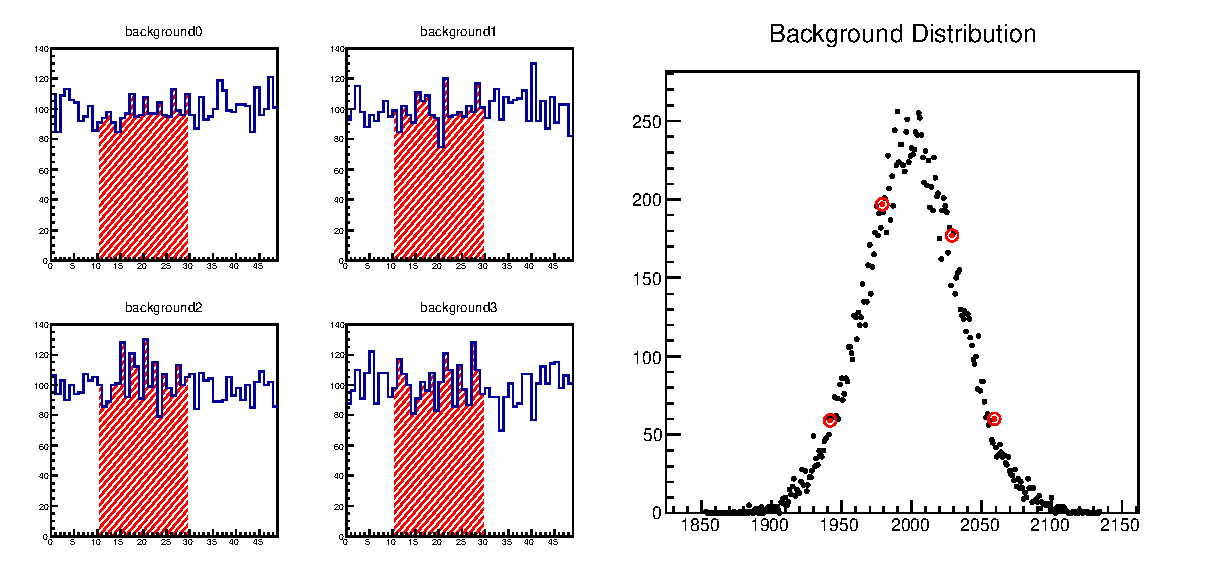
\includegraphics[width=0.3\textheight]{figures/bkgDist}
  \label{fig:bkgDist}}
  
  \subfloat[Distribution of Signal Counts][Distribution of Signal Counts]{
  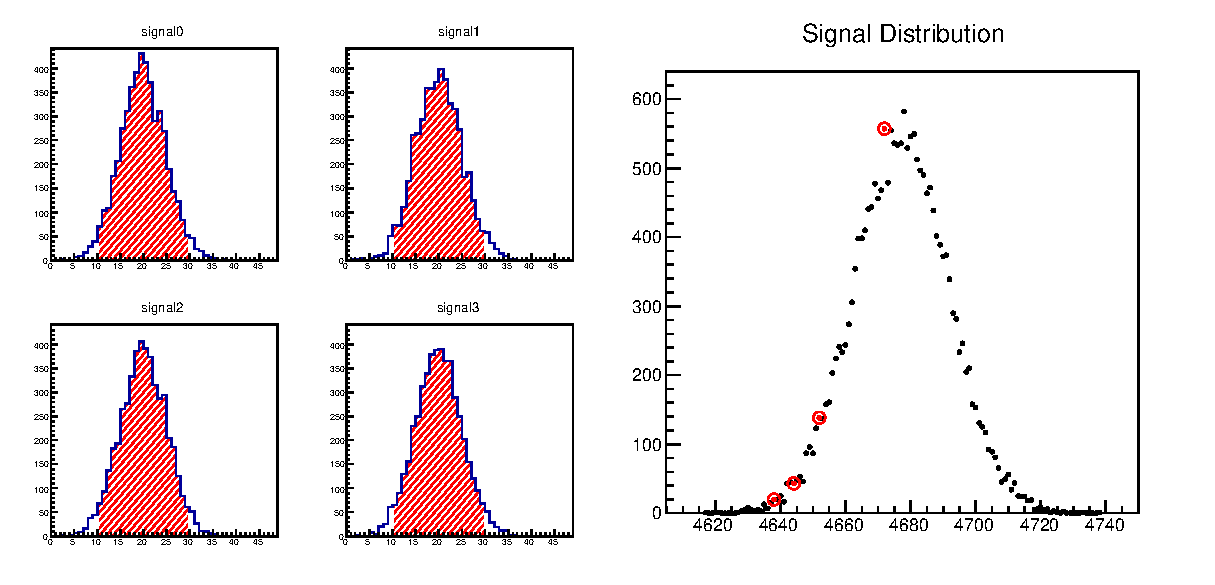
\includegraphics[width=0.3\textheight]{figures/sigDist}
  \label{fig:sigDist}}
  
  \subfloat[Distribution of Extracted Counts][Distribution of Extracted Counts]{
  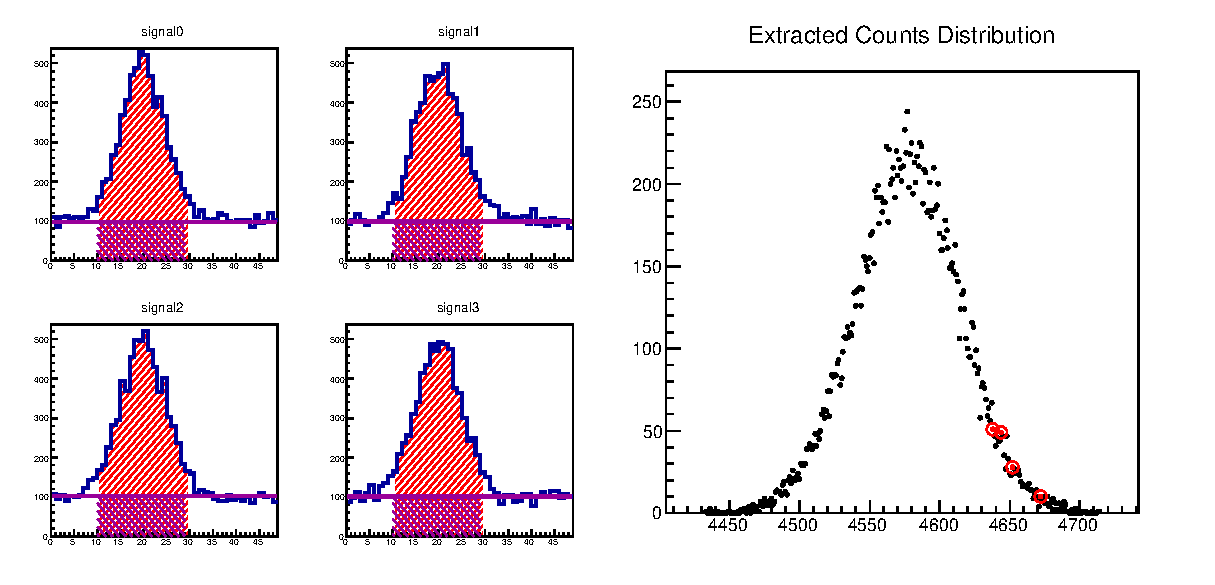
\includegraphics[width=0.3\textheight]{figures/extractDist}
  \label{fig:extractDist}}

  \caption{The number of counts in the peak region are a sum of the number of counts in the random background and counts from the neutrons.  The width of a sample at a uniform rate is simply $\sqrt{N}$, as seen in figure ??.  This is an appropriate description of the random background.  The neutron peak is roughly gaussian-shaped, and running trials where counts are drawn from a gaussian distribution shows that the width is ??.}
  \label{fig:statDist}
\end{figure}

The error introduced to the extracted counts depends on how the background is determined.  In the case of the pulse-selected data, it is clearly better to fit the background.  The constant component of the background is well-determined and contributes a tiny ??\% to the total error.  Next we estimate the uncertainty introduced by the evaporation spectrum.

A neutron continuum is clearly visible in all targets, and while in \Mg{26} the continuum is separated by ?? MeV, it is difficult to determine where the continuum for the \Se{76} and \Se{78} stops.  What is safe to assume is that neutrons populating the continuum cannot have an energy greater than the \zp neutron, and so its endpoint cannot extend past the center of the ground state neutron distribution.  Appropriate functional models, then, are those that are identically zero on an infinite or semi-infinite range.  Two functions that satisfy this criterion are the Beta Distribution and the Gamma Distribution, shown in {\fig}~\ref{fig:BetaGamma}.  The pulse-selected data set, however, does not constrain the tails of these functions well because the timing spectrum is not complete.  The non-pulse-selected data can help better constrain the fits in this region.

For the same bar, the pulse-selected spectrum should have the same shape as the non-pulse-selected data.  Fitting to the pulse-selected and non-pulse-selected histogram simultaneously greatly improves the fit.  The model for the pulse-selected data is
% equation for pulse-selected spectrum
\begin{equation}
Beta(A,B,\alpha,\beta) + Gaus() + Gaus() + Gaus() + DoubleGaus() + Const
\end{equation}
and for the non-pulse-selected data is
% equation for non-pulse-selected spectrum
\begin{equation}
Beta(A,B,\alpha,\beta) + Gaus() + Gaus() + Gaus() + DoubleGaus() + Const,
\end{equation}
where certainly the parameters of the Beta Distribution must be the same for each fit.  But these two histograms constrain each other in more ways than just the shape of the neutron evaporation spectrum.  A detector sitting at the same angle should see the same ratio between neutrons from the evaporation peak, neutrons from the Carbon peak, and neutrons from the \zp peak.  The full neutron spectra - peaks and evaporation region - from each of these histograms should have the same shape.  So now the model for the non-pulse-selected spectrum can be a neutron spectrum that's a scaled copy of the pulse-selected spectrum's neutron spectrum.  If we write the pulse-selected fitting function as 
% equation for pulse-selected spectrum
\begin{equation}
Neut_{PS} + DoubleGaus() + Const,
\end{equation}
then the form for the non-pulse selected data must be
% equation for non-pulse-selected spectrum
\begin{equation}
R*Neut_{PS} + DoubleGaus() + Const.
\end{equation}

Restricting the fixed scaling to the neutrons alone, however, is incorrect.  Bars of the neutron detector sit at a fixed angle and see the same mix of neutrons as well as the same mix of neutrons and gammas.  There are really two spectra the detector sees - a beam-related spectrum and the non-beam-related background spectra.  Two different runs will provide these in different ratios; for example, a short run with high beam current would proved more beam-related spectrum and little background spectrum, while a long run with low beam current would provide provide moderate beam-related spectrum and much background spectrum.  The appropriate model for fitting the two datasets simultaneously, then, is
% equation for pulse-selected spectrum
\begin{equation}
Neut_{PS} + Gamma_{PS} + Const_{PS}
\end{equation}
for the pulse-selected data and 
% equation for non-pulse-selected spectrum
\begin{equation}
R(Neut_{PS} + Gamma_{PS}) + Const_{NPS}
\end{equation}
for the non-pulse selected data.  That the gamma peaks scale by the same ratio as the neutron peaks is a significant constraint on this fit because they are such pronounced features.  Such a fit does indeed converge well for a large majority of the detectors and shows that the neutron evaporation spectrum contributes at most ??\% to the extracted counts in the ground-state neutron peak.  

The method used to extract the counts in the ground-state neutron peak is a direct summing of the counts from the peak region followed by subtraction of the estimated flat background from a linear fit.  The estimated error is the statistical error of the sum of the peak region and the systematic error of including counts from the continuum.  The results are plotted in {\fig}~\ref{fig:PS_angularDistribution}.

A dedicated fitter may begin to wonder if there are as-yet-unused constraints that could provide an even more robust fit that would ensure a convergent fit for all angles.  One additional constraint concerns the ratio between the two datasets.  This ratio scales the amount of beam seen by one bar during the two data runs.  But each bar should see the same ratio!  Fitting all the bars simultaneously will provide a much-improved ratio.

\subsection{Data with No Pulse Selection}
With pulse selection, the region behind the neutron peak has only random signal and can be fit with a constant to within ??\%.  With no pulse selection, the neutron peak sits on top of background from the previous bunch.  Fitting this spectrum by itself introduces significant uncertainty in the height of the evaporation spectrum because the flat background is not well-constrained by any portion of the spectrum.  The fit described above is a poor estimate of the background in the non-pulse-selected data because a wide range of shapes describing the evaporation continuum and random background produce good fits but very different estimated background in the ground-state neutron peak region.  Additionally, it becomes difficult to introduce enough peaks to accurately reproduce the shape of the background without making the fit unable to converge because there are too many independent variables. 

Instead of attempting to fit the non-pulse-selected background with a function, using the pulse-selected data itself as a template for the non-pulse-selected data is more accurate.  If the pulse-selected spectra are modeled as
\begin{equation}
Beam_{PS} + Const_{PS},
\end{equation}
then the non-pulse selected spectra can be understood as
% equation for non-pulse-selected spectrum
\begin{equation}
R\times (Beam1_{PS}+Beam2_{PS}+Beam3_{PS}) + Const_{NPS},
\end{equation}
where $Const_{PS}$, $R$, and $Const_{NPS}$ are free parameters and $Beam1_{PS}+Beam2_{PS}+Beam3_{PS}$ are shifted copies of the beam spectrum $Beam_{PS}$.  The beam-related component of the pulse-selected spectrum is a Kernel Density Estimate [CITE] based on the data in the histogram.  

Extraction of the ground-state neutron counts is done not by subtracting an estimated background from the total counts in the peak region, but rather by applying the ratio of signal to background to the total counts.  The results of the fits can be seen in {\fig}~\ref{fig:NPS_fits} and the final angular distribution in {\fig}~\ref{fig:NPS_angularDistribution}.


\section{Placing a Limit on Excited \zp States}
\begin{comment}
introduce 0+ peak and see when it becomes statistically significant
there will be different limits for different energies!  because of the evaporation background
\end{comment}
A primary aim of this experiment is to investigate the distribution of \zp strength, making it important to either measure or place a limit on the cross-sections of excited \zp states.  Because the non-pulse-selected data has significant, complicated background, only the pulse-selected data sets were used for this analysis.

No obvious \zp states were observed in the evaporation continuum for \Ge{74} or \Ge{76}.  A limit on the cross-section of \zp states as a function of energy can be determined by solving for the number of counts necessary to be consistent with zero at some certainty:
\begin{equation}
peak counts = i\sigma,
\end{equation}
or
\begin{equation}
\sigma(S) = i\sqrt{P+B}
               &\approxi\sqrt{S+B+B}
               &=i\sqrt{S+2B},
\end{equation}
where $S$ is the number of counts in the potential signal region and $B$ is the estimated number of counts.  In this case, sideband subtraction is the most appropriate method of determining $B$ because the shape of the continuum is not well-known and attempting to fit it functionally could introduce unknown systematic error.  The number of signal counts $S$ can be written as a function of the background counts $B$ and the desired level of certainty, $i$:
\begin{equation}
S = \frac{i^2 \pm \sqrt{i^4 + 8i^2B}}{2}.
\end{equation}

The $2\sigma$ limit on the cross-section for excited \zp states in \Ge{74} and \Ge{76} is shown in {\fig}~\ref{fig:zp_limit}.  The $2\sigma$ limit was chosen because we do not believe we had sensitivity to the $1\sigma$ limit, while a peak at the $3\sigma$ limit would have stood out clearly from the data.  A simulation of peaks at these limits is shown in {\fig}~\ref{fig:differentLimits}.

\section{Fitting 0+ ground state}
\begin{comment}
DWBA calculation
shell model
f$^2$, p$^2$ state strength ("form factor")
\end{comment}
As discussed in {\chap}~\ref{chap:nucl}, both the Cluster and Bayman-Kallio models typically describe the same shape for the $L=0$ angular distribution, but the Cluster model does not usually reproduce the absolute cross-section.  In the case of \GeTargets, however, the ratio between the cluster-model DWBA predictions and the experimentally obtained cross-section is on the order unity, as for the $^{58,60,62,64}$Ni isotopes, which are also f-p-g shell nuclei.  See {\tab}~\ref{tab:zpRatio} for the exact values.  That the cluster-model accurately predicts the \reaction cross-sections suggests two-step processes play a limited role in these reactions.

The cluster model can be sensitive to the parameters used to describe the potentials of the interacting nuclei.  The dependence of the cross-section for various \He{3} optical potential models was explored and were found to result in little difference in the elastic cross-sections.  See {\tab}~\ref{tab:parameterSensitivity} for the tested parameter ranges and {\fig}~\ref{fig:parameterSensitivity} for their impact on the relative cross-section.

The cross-sections measured for \reaction are consistent with DWBA predictions and data suggest no significant excited \zp states.
% % uncomment the following lines,
% if using chapter-wise bibliography
%
% \bibliographystyle{ndnatbib}
% \bibliography{example}
